Zur Umsetzung der Gestensteuerung eines Industrieroboters wird der Lernroboter WidowX 200, welcher zur InterbotiX X-Serie gehört und von Trossen Robotics hergestellt wird, als Vorlage für einen Industrieroboter verwendet. Mit seinen 5 DOF eignet sich der WidowX 200 für Testzwecke als sichere Alternative zu einem Knickarmroboter. Bei Tests geht im Gegensatz zu einem Industrieroboter eine geringere Gefahr vom WidowX 200 aus, da dieser keine so hohen Kräfte, Geschwindigkeiten und Beschleunigungen wie ein Industrieroboter entwickeln kann. Zudem bietet der \quoteMark{WidowX 200}-Lernroboter den Vorteil, dass es ein umfangreiches Dynamixel-SDK bietet, welches die Integration in ROS und die direkte Kommunikation mit dem Lernroboter einfach gestaltet und daher die Entwicklung des für Gestensteuerung konzipierten Systems drastisch beschleunigt. Für den Gelenk-Modus stellt der Lernroboter auch die Möglichkeit bereit die Gelenke individuell ansprechen und deren Gelenkposition verändern zu können. Die Dynamixel-Servo-Motoren können individuell an die Befürfnisse der Aufgabenstellung angepasst werden, da unter anderem die maximale Geschwindigkeiten und Beschleunigungen der einzelnen Servo-Motoren individuell konfigurierbar sind. Die Reichweite des Roboterarms beträgt in eine Richtung \num{55} cm. Der Arbeitsbereich des WidowX 200 ist kreisförmig und liegt bei einem Durchmesser von \num{110} cm. Im Arbeitsbereich des WidowX 200 sollten sich keine ungewollten Objekte befinden und sichergestellt werden, dass der WidowX 200 in diesem Bereich frei von menschlichen Einflüssen bewegen kann. Anzumerken ist, dass die Wiederholgenauigkeit des WidowX 200 bei \num{1} mm liegt. Für individuelle Aufgabenstellungen kann der Endeffektor jederzeit durch bereits verfügbare oder selbst z.B. durch einen per 3D-Druck erstellten Endeffektor ersetzt werden. Das maximale Tragegewicht des WidowX 200 beträgt 200 g, welches nicht überschritten werden sollte, da ansonsten Fehler bei der Änderung der Gelenkposition auftreten können \cite{widowx_200_nodate}.\\

Zur Gestenerkennung wird die Azure Kinect aufgrund der eingebauten Tiefenkamera verwendet. Auf die Azure-Cloud-Integration wird jedoch verzichtet, da das Azure Kinect Body Tracking SDK durch ein DNN eine ausreichend genaue Methode bereitstellt \cite{qm13_azure_kinect_release_notes_nodate} um 32 spezifische Positionen des menschlichen Körpers, zu denen unter anderem die Augen, Schulter, Knie, Daumen und Zeigefinger zählen, zu erkennen \cite{qm13_azure_joints_nodate}. Zudem wird durch den Einsatz des Azure Kinect Body Tracking SDK die Entwicklung des für Gestensteuerung konzipierten Systems drastisch beschleunigt. Einzelne Finger können aufgrund der Limitierung des Azure Kinect Body Tracking SDKs und der verbauten Tiefenkamera der Azure Kinect allerdings nicht erfasst werden. Gesten, welche jedoch die Hand im Allgemeinen beinhalten, wie z.B. die Stopp-Geste, sind dagegen unter anderem durch die vorhandenen räumlichen Positionsinformationen realisierbar \cite{microsoftazure-kinect-sensor-sdk_2020}.\\

Die Gestensteuerung des WidowX 200, welches auf dem für diese Arbeit erstellten Roboter-Gesten-Framework basiert und als Basis für andere gestengesteuerte Roboter dienen kann, wird näher beschrieben und verschiedene Gesten werden nach der Ergonomie evaluiert. Anschließend werden Gesten, welche mit der Azure Kinect umsetzbar sind, ausgewählt und mit Sicherheitsvorkehrungen kombiniert, welche es verhindern sollen, dass der Roboter sich unbeabsichtigt bewegt.

% https://elib.uni-stuttgart.de/bitstream/11682/9072/1/Schneider-Dissertation-60.pdf
% https://robodk.com/doc/de/Robot-Validation-ISO9283.html

\section{Allgemeine Anforderungen}
Um die Gestensteuerung des WidowX 200 bewerten zu können müssen die allgemeinen Anforderungen an die Software zur Gestensteuerung eines Industrieroboters aufgezeigt werden. Hierzu zählen die funktionalen sowie auch die nichtfunktionalen Anforderungen an die Software zur Gestensteuerung eines Industrieroboters.

\subsection{Funktionale Anforderungen}
Die Anforderungen an die Software zur Gestensteuerung eines Industrieroboter können in die nachfolgenden Punkte gegliedert werden \cite{kircher_it_2006} \cite[2\psq]{brauer_gestenerkennung_nodate}:\\

\begin{compactitem}
    \item \textbf{Nutzung von verbreiteten Paradigmen für die Entwicklung}: Um mehrere Komponenten, welche auf unterschiedlichen Systemen verteilt sein können, miteinander kommunizieren lassen zu können bedarf es eines gemeinsamen Konzepts. Bei Industrierobotern wird hierbei vermehrt ROS eingesetzt, welches es erlaubt ROS-Messages über ein Netzwerkprotokoll verschicken zu können.
    \item \textbf{Standardisiertes Austauschformat}: Der Austausch der Informationen kann bei ROS über sogenannte ROS-Messages erfolgen und beim Speichern und Laden von Informationen in ein standardisiertes Austauschformat, wie z.B. JSON oder XML, übersetzt werden. Hierdurch kann die Interoperabilität zwischen den Systemen gewährleistet werden.
    \item \textbf{Zuverlässigkeit der Übertragung}: Die ROS-Messages müssen unverändert und vollständig über das Netzwerk an den ROS-Master geschickt werden können. Hierfür wird zumeist TCP/IP als Netzwerkprotokoll eingesetzt, welches die vollständigkeit und richtige Reihenfolge der zugrundeliegenden Datenpakete gewährleistet.
    \item \textbf{Zuverlässigkeit der Gestenerkennung}: Die Gestensteuerung sollte eine möglichst kleine Falsch-Positiv-Rate aufweisen um unbeabsichtigte Gesten möglichst gering zu halten und so gefährlichen Situationen entgegenwirken zu können.
    \item \textbf{Echtzeitfähigkeit}: Das System muss sicherstellen, dass es die Informationen in einem gewissen Zeitintervall abarbeiten kann um die Sicherheit des Systems und der beteiligten Menschen gewährleisten zu können.
    \item \textbf{Adaptionsmöglichkeit an verschiedene Tiefenkameras}: Es muss die Möglichkeit bestehen im System die Tiefenkamera durch eine andere Tiefenkamera austauschbar zu machen. Hierbei muss sichergestellt werden, dass die Tiefenkameras die gleichen Schnittstellen verwenden um die gleiche Kommunikation zu ermöglichen.
    \item \textbf{Adaptionsmöglichkeit an verschiedene Industrieroboter}: Durch die schiere Anzahl an Industrierobotern muss es zudem auch möglich sein den Industrieroboter durch einen anderen Industrieroboter, unabhängig von seiner bisher vorhandenen Schnittstellen, ersetzen zu können.
    \item \textbf{Ergonomische Gesten}: Die Gesten müssen leicht erlernbar, einfach anwendbar und leicht zu erlernen sein. Zudem sollte ein längeres Verwenden der Gesten höchstens zu geringen Ermüdungserscheinungen führen und das System von Links- sowie auch Rechtshändern bedienbar sein.
    \item \textbf{Genauigkeit der Erreichung der Zielpose}: Die Zielpose muss je nach Genauigkeit des Industrieroboters über die Gestensteuerung erreichbar sein. Ungenauigkeiten durch die Gestensteuerung, welche aber auch bei Teach Pendants vorhanden sind, sind subjektiver Natur.
    \item \textbf{Sicherheitsvorkehrungen}: Es muss sichergestellt werden können, dass der Industrieroboter jederzeit durch einen Notstop unverzüglich gestoppt werden kann um lebensbedrohliche Situationen vorbeugen zu können.
\end{compactitem}

\subsection{Nichtfunktionale Anforderungen}
Da in dieser Arbeit das Roboter-Gesten-Framework mit und ohne ROS lauffähig sein soll, müssen die Anforderungen an die Schnittstelle zwischen dem Industrieroboter und der Tiefenkamera genauer spezifiziert werden. Die Anforderungen an die Schnittstelle zwischen dem Industrieroboter und der Tiefenkamera sind daher die Folgenden, welche aufgrund von ROS den Anforderungen von Server-Client-Anwendungen entsprechen \cite{osterrieder_komponentenmodelle_2004}:\\

\begin{compactitem}
    \item \textbf{Performanz}: Bei der Kommunikation zwischen den einzelnen Systemen, zu denen die Tiefenkamera und der Industrieroboter zählen, sollte die Anfrage so schnell wie möglich erfolgen, ohne lange Wartezeiten zu benötigen.
    \item \textbf{Zuverlässigkeit}: Die Zuverlässigkeit beschreibt, wie verlässlich ein System seine Aufgaben ausführt. Ausfälle von ROS-Nodes oder sogar des ROS-Masters selbst reduzieren hierbei unter anderem die Zuverlässigkeit des Systems drastisch.
    \item \textbf{Modularität}: Spiegelt den Grad der Aufteilung in Komponenten wider, welche vom eigenen Projekt oder von Dritten wiederverwendet werden können.
    \item \textbf{Erweiterbarkeit}: Bezeichnet die Fähigkeit des Systems durch weitere Komponenten, welche dem System hinzugefügt werden können, angepasst zu werden. Bei ROS können zusätzliche ROS-Packages von Drittanbietern installiert werden, wodurch das System erweitert werden kann.
\end{compactitem}

\section{Einrichtung des Testsystems}
Zur Umsetzung der Gestensteuerung von Industrierobotern wird ROS 1 mit dem Codenamen Melodic Morenia, welches als LTS-Version verfügbar ist und daher Langzeitunterstützung bietet, eingesetzt \cite{robot_operating_system_2020}. Als Betriebssystem kommt Ubuntu 18.04 Bionic Beaver zum Einsatz, da dies die neueste unterstützte LTS-Version von Ubuntu darstellt, welche von ROS Melodic Morenia empfohlen wird \cite{ros_distributions_nodate}.

\subsection{Linux-Container}
Zur besseren Einsetzbarkeit auf unterschiedlichen Linux-Distributionen wird das genannte Ubuntu 18.04 Bionic Beaver und ROS Melodic Morenia in einem Linux-Container installiert und per Image zur Verfügung gestellt. Der Vorteil durch die Container-Technik stellt hierbei das einfachere und schnellere Deployen, der in dieser Arbeit entwickelten Anwendung zur Gestensteuerung des WidowX 200, dar. Zudem bietet die Container-Technik im Gegensatz zu einem Hypervisor, wie z.B. VMware, VirtualBox oder Hyper-V, den Vorteil, dass kein vollständiges Linux-Betriebssystem virtualisiert werden muss, welches einen impliziten Ressourcen-Overhead, wie z.B. hohe RAM- und CPU-Auslastung, mit sich ziehen würde. Zur Umsetzung der Trennung von Prozessen werden die Kernelnamensräume und für die Ressourcenverwaltung cgroups eingesetzt, welche im Linux-Kernel enthalten sind. Dies führt dazu, dass der Linux-Container auf den gleichen Kernel wie das Host-System zugreifen kann, jedoch aber der Zugriff auf sensible Ressourcen durch den Linux-Kernel beschränkt oder sogar vollständig untersagt wird \cite{lxc_2020}. Linux-Container werden auch kurz LXC genannt, welches auch die gleichnamige Bezeichnung für das Userspace-Tool ist um die Linux-Container zu verwalten. Die Erweiterung von LXC wird LXD genannt und ermöglicht die Verwaltung von mehreren LXC-Instanzen über einen System-Daemon, welcher per REST-API angesprochen werden kann. Zudem bietet LXD unter anderem die Möglichkeit Snapshots von Linux-Containern zu erstellen, zu erzeugen, zu starten und zu stoppen \cite{lxc_2017}. Für diese Arbeit wird als Host-System, auf dem die LXC-Instanz installiert und ausgeführt wird, Ubuntu 20.04 Focal Fossa verwendet, welches eine LTS-Version von Ubuntu ist und die den Linux-Kernel 5.4 einsetzt. Andere Linux-Distributionen sind grundsätzlich auch möglich solange die für diese Arbeit benötigten Features im Linux-Kernel verfügbar sind. Die entwickelte Roboter-Gesten-Anwendung wird im Linux-Container mit echtzeitfähiger Priorität ausgeführt, da die maximale Latenz des Kommunikationskanals des Eingabegerätes aufgrund der Maschinenrichtlinien 2006/42/EG und der \quoteMark{ISO EN 10218}-Norm weniger als 50 ms betragen und zudem ein deterministisches Verhalten aufweisen muss \cite[55]{prassler_advances_2004}. Die benötigten Features des Linux-Kernels und zudem das Einrichten des Linux-Schedulers, welcher feste Echtzeitfähigkeit garantieren muss, können zudem aus der Installationsanleitung, welche sich im Anhang \ref{appendix1:Einrichtung_des_Testsystems} befindet, entnommen werden.

% https://www.techdivision.com/blog/lxc-vs-docker-wir-setzen-bei-techdivision-inzwischen-verstaerkt-auf-lxc.html
% https://www.linux-magazin.de/ausgaben/2015/05/lxd/

\subsection{Simulationsumgebungen}
Zum Durchführen von Tests werden oft Simulationsumgebungen verwendet, da diese den Vorteil bieten, dass kein realer Roboter vorhanden sein muss und dadurch gefährliche Situationen für den Menschen erst gar nicht entstehen können. Während der Entwicklung eines Roboters kann dieser sogar in einer virtuellen Umgebung getestet werden um so das Verhalten und technische Limitierungen des Roboters vor der Herstellung zu ermitteln. Dies spart Zeit und Kosten, da das fertige Produkt erst nach ausführlichen Tests hergestellt wird. Mit Simulationsumgebungen können zudem Tests schneller und effizienter durchgeführt werden, da unter anderem Differenzen zu exakten Zielposen einfacher und genauer als mit manuellen Messungen bestimmt werden können \cite{gazebo_nodate}. Zwei der bekanntesten Simulationsumgebungen, welche frei auf dem Markt verfügbar sind und unterschiedliche Roboter unterstützen, sind Gazebo und Coppelia Sim, welches der Nachfolger von vRep darstellt. Beide Simulationsumgebungen sind unter Windows, Linux und macOS verfügbar und bieten die Möglichkeit die standardmäßige Physik-Engine nach belieben mit einer anderen Physik-Engine auszutauschen um z.B. eine genauere Simulation durchführen zu können. Copellia Sim und Gazebo besitzen zudem beide einen Szenen-Editor und bei Coppelia Sim ist zudem im Gegensatz zu Gazebo ein 3D-Model-Editor integriert. Bei Gazebo wird hierdurch eine externe Anwendung benötigt um die 3D-Modelle den jeweiligen Bedürfnissen anpassen zu können. Coppelia Sim ist zudem aufgrund der Stabilität der GUI und der Plugins und der besseren Dokumentation im Gegensatz zu Gazebo zu bevorzugen. Viele Roboter werden aufgrund der ROS-Integration standardmäßig mit Out-of-the-Box-Unterstützung für Gazebo ausgestattet, wodurch bei Verwendung von Coppelia Sim zumeist ein Mehraufwand zum Einrichten des Roboters vonnöten ist. Beide Simulationsumgebungen bieten die Möglichkeit an über ROS-Messages angesprochen zu werden. Hierdurch ist eine Integration in ROS leicht umsetzbar. Copellia Sim und Gazebo bieten jedoch aber auch die Möglichkeit an vollständig ohne ROS verwendet werden zu können und so in beliebigen Softwareumgebungen eingesetzt zu werden \cite{vrep_vs_gazebo_nodate}. In dieser Arbeit wird Gazebo eingesetzt, da bereits der \quoteMark{WidowX 200}-Lernroboter eine vollständige Gazebo-Unterstützung mitliefert. Die benötigten Schritte zum Einrichten der Simulationsumgebung für den \quoteMark{WidowX 200}-Lernroboter können aus dem Anhang \ref{appendix1:Einrichtung_des_Testsystems} entnommen werden.

% https://www.ros.org/integration/
% http://gazebosim.org/
% https://www.coppeliarobotics.com/features

\section{Anbindung an ROS}
Da Gazebo standardmäßig eine ROS-Integration bereitstellt müssen nur die ROS-Packages des \quoteMark{WidowX 200}-Lernroboters installiert werden um die Gazebo-Integration einzurichten, wie aus dem Anhang \ref{appendix1:Einrichtung_des_Testsystems} zu entnehmen ist. Die Simulationsumgebung kann daraufhin gestartet und z.B. für Testzwecke genutzt werden. Die ROS-Packages des \quoteMark{WidowX 200}-Lernroboters werden von Trossen Robotics entwickelt und der Quellcode kann öffentlich eingesehen werden um eigene Anpassungen daran durchführen zu können. Der \quoteMark{WidowX 200}-Lernroboter kann aufgrund des \quoteMark{InterbotiX}-Nodes von überall aus dem Roboter-Netzwerk angesprochen werden. Zudem ist durch die ROS-Unterstützun des WidowX 200 überhaupt erst möglich MoveIt zu unterstützen. MoveIt ist ein ROS-Package, welches es vor allem ermöglicht Bewegungen zu Planen, die inverse und direkte Kinematik zu berechnen oder aber auch Kollisionschecks mit einem Tiefensensor zu ermöglichen \cite{moveit_nodate}. Zudem bietet MoveIt eine C++-API an um die ROS-Services zu überspringen und eine höhere Performanz als mit einer vollständigen ROS-Umsetzung zu erhalten \cite{moveit_tutorial_nodate}.\\

Für das Azure Kinect Sensor SDK, welches direkten Zugriff auf die Sensoren der Azure Kinect ermöglicht, und das Azure Kinect Body Tracking SDK, welches zur Gestenerkennung eingesetzt werden kann, werden keine ROS-Packages von Microsoft bereitgestellt \cite{tesych_about_azure_kinect_sdks_nodate}. Daher ist es notwendig diese direkt in einen eigenen ROS-Node oder direkt in den ROS-Node der in dieser Arbeit entwickelten Roboter-Gesten-Anwendung zu integrieren. Aufgrund der Komplexität der Gestenerkennung, der Notwendigkeit zur schnellen und sicheren Reaktion auf die Gesten und der Möglichkeit von sehr schnell aufeinander folgenden Gesten und Bewegungsabläufen der Hände wurde entschieden die Gestenerkennung über eine C++-Schnittstelle bereitzustellen um möglichst jederzeit sicherstellen zu können, dass die Nutzereingaben schnell genug an die Steuereinheit übermittelt werden können. Zudem bietet es bei der Messung der Latenz der Übertragung mit und ohne ROS-Anbindung den Vorteil, dass schnell darauf geschlossen werden kann wo der Flaschenhals im System liegt. Dies wäre mit sehr vielen selbst erstellten und verteilten ROS-Nodes nur sehr schwer bis überhaupt nicht einsehbar, da das System zu komplex werden würde \cite{why_dont_we_use_ros_nodate}. Der ROS-Node zur Gestenerkennung muss durch diesen Ansatz nur noch die benötigten Roboter-Befehle per MoveIt oder über die ROS-Schnittstelle des Industrieroboters an die Motoren des Industrieroboters senden um Gelenkbewegungen auslösen zu können.

\section{Gesten}
Zu Gesten zählen alle Formen der Bewegung, welche der nonverbalen Kommunikation dienen und mit den Armen, den Händen, dem Kopf, den Füßen oder Beinen ausgeführt werden können \cite{gestik_2020}. Wissenschaftler unterscheiden bis zu 5000 verschiedene Gesten, welche weltweit bewusst oder unbewusst eingesetzt werden. Handgesten werden vor allem dafür eingesetzt um Aussagen zu untermauern und deren Wirksamkeit zu verstärken. Bei Gesten sind auch die verschiedenen Posen des eingesetzten Körperbereichs entscheident zu beachten, da die Geste je nach Pose unterschiedliche Bedeutung besitzen kann. Z.B. ist das Greifen des Kinns mit dem Zeigefinger und Daumen eine nachdenkliche Geste, welche jedoch durch überdecken des verschlossenen Mundes mit dem Zeigefinger zu einer anderst interpretierbaren Geste wird. Das Überdecken des verschlossenen Mundes mit dem Zeigefinger kann als ein bewusstes Unterdrücken von Informationen angesehen werden und spiegelt daher nicht mehr die nachdenkliche Pose wider \cite[137\psq]{matschnig_korpersprache_2007}.

\subsection{Arten von Gesten}
Je nach Religion, Situation, Kultur, sozialer Herkunft, unterschiedlicher Ansichten und je nach Gefühlslage können Gesten eine andere Bedeutung besitzen. Aus diesen Gründen ist es sehr wichtig die verschiedenen Arten von Gesten zu kennen um so möglichst ethisch neutrale Gesten für die Kommunikation mit einem Industrieroboter auswählen zu können \cite{gesten_liste_2020}. Daraus wird ersichtlich, dass nicht nur die Geste selber für das interpretieren notwendig ist, sondern aber auch der Kontext in der die Geste eingesetzt wird. Je nach Kontext sind körpernahe und körperferne Gesten, welche z.B. zum Zeigen auf Objekte eingesetzt werden, daher gleichermaßen für Missinterpretationen anfällig \cite[137\psq]{matschnig_korpersprache_2007}, da z.B. beim Erschrecken die Hände reflexartig ausgestreckt werden, bei Angstzuständen oder starker Wärme der Schweiß von der Stirn gewischt oder bei Rückenschmerzen an den Rücken gegriffen wird \cite{matschnig_glossar_nodate}.\\

\begin{figure}[!h]
    % Set the overall layout of the tree
    \tikzstyle{level 1}=[level distance=1.6cm, sibling distance=8.5cm]
    \tikzstyle{level 2}=[level distance=1.6cm, sibling distance=3.5cm]
    \tikzstyle{level 3}=[level distance=1.6cm, sibling distance=5.2cm]
    \tikzstyle{level 4}=[level distance=1.6cm, sibling distance=2.8cm]

    % Define styles for bags and leafs
    \tikzstyle{bag} = [draw=none, fill=none, text centered]
    \tikzstyle{end} = [draw=none, fill=none, text centered]

    \centering
    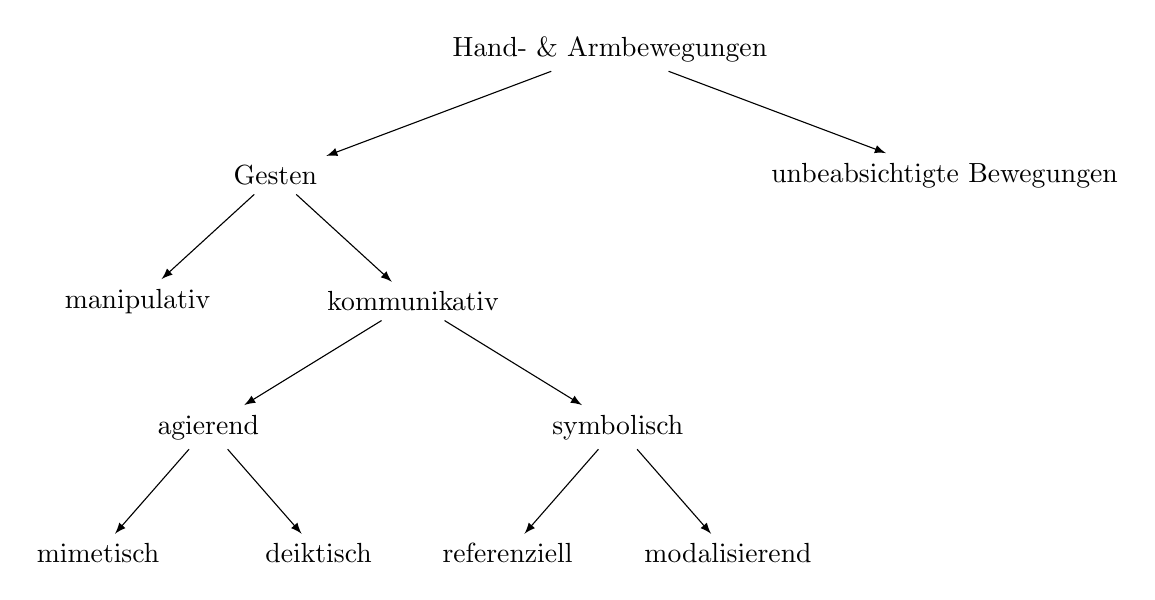
\begin{tikzpicture}[grow=down, sloped, edge from parent/.style={draw,-latex}]
    \node[bag] {Hand- \& Armbewegungen}
        child {
            node[bag] {Gesten}
                child {
                    node[end] {manipulativ}
                }
                child {
                    node[bag] {kommunikativ}
                        child {
                            node[bag] {agierend}
                                child {
                                    node[end] {mimetisch}
                                }
                                child {
                                    node[end] {deiktisch}
                                }
                        }
                        child {
                            node[bag] {symbolisch}
                                child {
                                    node[end] {referenziell}
                                }
                                child {
                                    node[end] {modalisierend}
                                }
                        }
                }
        }
        child {
            node[end] {unbeabsichtigte Bewegungen}
        };
    \end{tikzpicture}\newline
    \caption[Einteilung der Gesten]{Einteilung der Gesten\\Quelle: Eigene Darstellung, in Anlehnung an \cite[680]{pavlovic_visual_1997}}
	\label{fig:einteilung_der_gesten}
\end{figure}
\FloatBarrier

Eine der bekanntesten Gesten-Taxonomien für HCI mit denen alle Hand- und Armbewegungen, welche in Abbildung \ref{fig:einteilung_der_gesten} ersichtlich sind, klassifiziert werden können, stammt von F.K. Quek, einem  Professor für Informatik und Mathematik am Virginia Polytechnic Institute und der State University. Diese Taxonomie teilt die Hand- und Armbewegungen in Gesten und unbeabsichtigte Bewegungen ein. Nur wenn die Geste mit einer absichtlichen Hand- oder Armbewegung durchgeführt wurde, wird die Hand- oder Armbewegung in diesem Modell als Geste klassifiziert. Alle anderen Hand- oder Armbewegungen sind daher nach diesem Modell keine Gesten, da diese für den Computer keine sinnvollen Informationen bieten. Gesten können nach dieser Taxonomie wiederum in manipulative und kommunikative Gesten unterteilt werden. Manipulative Gesten werden dazu verwendet mittels z.B. Bewegungsgesten oder Drehgesten auf Objekte in der Umgebung einzuwirken und diese zu verändern, wohingegen kommunikative Gesten einen inhärenten kommunikativen Zweck erfüllen und zumeist durch die Sprache unterstützt werden. kommunikative Gesten können wiederum in agierende und symbolische Gesten unterteilt werden. Der Unterschied zwischen symbolischen und agierenden Gesten besteht darin, dass symbolische Gesten im Gegensatz zu agierenden Gesten eine bildliche Beschreibung einer Aktion darstellen und mit einer zuvor definierten Aktion verknüft werden müssen um diese interpretierbar zu machen. Agierende Gesten stehen hingegen im direkten Zusammenhang mit der Aktion und deren Auswirkung ist daher auch direkt erkennbar. Die referenzielle Geste, welche zur symbolischen Gestenart zählt, kann z.B. eine kreisförmige Bewegung mit dem Zeigefinger sein, welche angibt dass die Bewegung auf ein Rad bezogen ist und dieses sich bewegen soll. Neben der referenziellen Geste existiert auch die modalisierende Geste, welche im Gegensatz zur referenziellen Geste eine Aktion durch eine symbolische Geste und zusätzlicher Verwendung der Sprache vorgibt. Bei symbolischen Gesten sind daher der Kreativität keine Grenzen gesetzt und deshalb können diese Gesten nach belieben mit verschiedenen Aktionen verknüpft werden. Zu den agierenden Gesten zählen mimetische und deiktische Gesten, welche im direkten Zusammenhang mit der Interpretation der Geste stehen. Deiktische Gesten werden dabei mit dem Zeigefinger durchgeführt und geben z.B. eine Position vor, wohingegen mimetische Gesten bestimmte Aktionen imitieren. Im HCI-Kontext werden überwiegend symbolische Gesten eingesetzt, da diese zumeist durch verschiedene statische Handhaltungen dargestellt werden können und so zumeist anstrengende und ermüdende Gesten vermeiden \cite[680]{pavlovic_visual_1997}.

% https://toastmasters-dortmund.de/wp-content/uploads/Gesten-Ihr-K%C3%B6rper-spricht.pdf
% S. 8

% https://www.uni-bremen.de/fileadmin/user_upload/sites/artec/Publikationen/artec_Paper/042_paper.pdf

% Semaphorische  Gesten (Körperhaltung)   https://tu-dresden.de/ing/informatik/smt/mg/ressourcen/dateien/studentische-arbeiten/2011_beleg_herrmann.pdf?lang=de
% dynamische und statische Gesten -> statische Gesten

% https://pdfs.semanticscholar.org/a214/7d3db5335383d4db53e68ffcadbdc66b9568.pdf
% S. 68

% http://campar.in.tum.de/pub/walchshaeusl2004da/walchshaeusl2004da.pdf
% S. 7

% https://edoc.sub.uni-hamburg.de//haw/volltexte/2017/4014/pdf/graczyk_bachelorarbeit.pdf

\subsection{Beispiele für unethische symbolische Gesten}
Gesten können je nach Religion, Situation, Kultur, sozialer Herkunft, unterschiedlicher Ansichten und je nach Gefühlslage auf eine andere Art und Weise interpretiert werden. Die auszuwählenden Gesten sollten daher für alle Menschen ethisch vertrettbar sein um Missverständnissen und peinlichen Momenten vorzubeugen \cite{gesten_liste_2020}. Aus diesem Grund werden hierfür beispielhaft ein paar Gesten aus aller Welt miteinander verglichen und deren Bedeutungen in den unterschiedlichen Ländern erklärt.\\

\textbf{Daumen hoch}: Die \quoteMark{Daumen hoch}-Geste wird im deutschsprachigen Raum, USA und Korea dazu verwendet um eine besondere Leistung hervorzuheben. In anderen Ländern, wie z.B. Russland, Frankreich, Israel, Griechenland und Italien, ist es jedoch eine obszöne Aufforderung zum Sex und sollte daher nicht verwendet werden um eine unangenehme Situation und daraus resultierende Probleme zu vermeiden. In China und Japan hingegen bedeutet die \quoteMark{Daumen hoch}-Geste, dass man fünf Stück von einer Sache bestellen will und in Japan kann es zudem auch als Synonym für einen festen Freund missinterpretiert werden. Die \quoteMark{Daumen hoch}-Geste kann in Australien, Afghanistan, Iran, Irak und Nigeria auch als provokante Aufforderung zum Gehen missverstanden werden \cite{handzeichen_gesten_2018}.\\

\textbf{Daumen-Zeigefinger-Kreis}: Die \quoteMark{Daumen-Zeigefinger-Kreis}-Geste wird im deutschsprachigen Raum, Nordamerika/USA, England, Mexiko, Skandinavien und Kanada positiv aufgefasst und bedeutet in den meisten Fällen \quoteMark{Okay} oder, dass zumeist ein Aufgabe sehr gut ausgeführt wurde. In der Türkei, Griechenland und Russland zeigt man hierdurch symbolisch eine Körperöffnung, welche in diesen Ländern als obszön zu betrachten ist. Die \quoteMark{Daumen-Zeigefinger-Kreis}-Geste wird in Brasilien als obszöne Beleidung aufgefasst und in Belgien und Tunesien wird damit sogar ausgedrückt, dass die andere Person eine Null und dadurch nutzlos ist \cite{handzeichen_gesten_2018}.\\

\textbf{Zeigefinger ausstrecken}: Das Richten des Zeigefingers auf andere Personen ist in den meisten Ländern, wie z.B. dem deutschsprachigen Raum, Frankreich, Italien, China und Japan, ein Zeichen der Respektlosigkeit und der Verachtung. Wenn der Zeigefinger auf sich selbst gezeigt wird, stellt es hingegen ein Zeichen der eigenen Selbstverliebtheit dar, welches in den genannten Ländern, wie auch das Zeigen mit dem Zeigefinger auf andere Personen, als negativ zu werten ist \cite{gesten_vergleich_nodate}.\\

\textbf{Mit Zeigefinger an die Stirn tippen}: Im deutschsprachigen Raum wird diese Geste als sehr abwärtend wahrgenommen und bedeutet im Normalfall, dass die andere Person ein Idiot ist. In Nordamerika und Peru hingegen ist es eine Anerkennung und ein Ausdruck dafür, dass die andere Person sehr schlau bzw. clever ist. In den USA wird diese Geste sogar dazu verwendet um andere Personen im Straßenverkehr freundlicherweise darauf hinzuweisen, dass in der Nähe eine Polizeikontrolle stattfindet \cite{handzeichen_gesten_2018}.\\

Im Großen und Ganzen kann resultierend gesagt werden, dass es nur schwer möglich ist Gesten so zu gestalten damit sie für alle religiösen, kulturellen und sozialen Gegebenheiten und in jeglichem Kontext frei von Missinterpretationen sind. Es ist jedoch möglich die Gesten aufgrund der bisher erarbeiteten Grundlage weitgehend ethisch zu gestalten und auszuwählen um möglichen Missinterpretationen entgegenwirken zu können.

% https://www.diepresse.com/5507147/gefahrliche-gesten#slide-2
% https://www.redenwelt.de/rede-tipps/gesten-im-ausland/

% https://tu-dresden.de/ing/informatik/smt/cgv/die-professur/mitarbeiter/ludwig_schmutzler/ludwig_schmutzler_ws1213

% „Designing Gestural Interfaces: Touchscreens and Interactive Devices“[Saffer, 2009, ab S. 183]

\subsection{Auswahl anhand der Ergonomie}
Aufgrundlage der ermittelten Limitierungen der Azure Kinect und der untersuchten ethischen Voraussetzungen können nun entsprechende Gesten entwickelt werden, welche die Anforderungen an die sicherheitskritische Steuerung eines Industrieroboters zur Vermeidung von Unfällen erfüllen. Zudem müssen die Gesten auch aus ergonomischer Sicht einfach und angenehm ausführbar sein und im besten Fall während des Teachens keine großen Ermüdungserscheinungen aufweisen. Um dies zu erreichen ist es unter anderem notwendig möglichst leicht zu merkende Gesten anstatt komplizierter Gesten zu wählen, da hierdurch die Erlernbarkeit der vorhandenen Gesten vereinfacht wird \cite[97]{schleicher_einfuhrung_2020}. Aus Gründen der Ergonomie sind Freihandgesten mit ausgestreckten Armen möglichst zu vermeiden, wenn diese auf Dauer ausgeführt werden müssen, da diese schnell zu Ermüdungserscheinungen führen \cite[84]{neupert_naturliche_nodate}. Eine direkte und natürliche Interaktion, welche intuitiv und einfach gestaltet ist, steigert zudem die Zufriedenheit der Personen, welche die Gesten einsetzen müssen \cite[103]{schleicher_einfuhrung_2020}. Zudem ist eine ausreichende Rückmeldung des Gestensystems praktisch, da hierdurch die Zufriedenheit der bedienenden Person und dessen Vertrauen zum System gesteigert wird \cite[132\psq]{schleicher_einfuhrung_2020}. Im Gegensatz zu VR oder AR können beim Verzicht auf diese Technologien keine virtuellen Objekte, wie in AR in der realen Umgebung oder wie bei VR in einer virtuelle Umgebung, platziert werden um der bedienenden Person z.B. eine Hilfestellung zur Verwendung der Gestensteuerung zu geben. In AR und VR wäre es möglich z.B. ein Tutorial bereitzustellen, welches die Bewegungsbahnen und Gesten in der jeweiligen Umgebung einblendet. Die bedienende Person hätte dann die Möglichkeit diese Gesten nachzuahmen und die Bedienung spielerisch zu erlernen \cite{weidenhausen_mobile_2007}. Eine gute Benutzererfahrung ist aber auch damit verbunden, dass das System die Gesten zuverlässig genug erkennt und die Gesten während des Einsatzzweckes für die bedienende Person nicht zu anstrengend werden. Zudem sind Gesten im Oberkörperbereich zu bevorzugen, da mit den Händen und Armen in diesem Bereich ohne die Arme übermäßig strecken zu müssen, verschiedene Bewegungen möglich sind \cite{nowack_pdf_2017}. Bei kurzen Aufgabenstellungen von wenigen Sekunden können Freihandgesten gewählt werden, da diese auf kurze Zeitspannen nicht anstrengend sind. Auf längere Sicht wirken die Freihandgesten jedoch ermüdend auf die bedienende Person, da es sehr anstrengend sein kann die Hand vom Körper weg zu halten \cite{krammling_user_2018}. Die Hand muss zudem über eine längere Zeitdauer hinweg, genau nach den Anforderungen des Gestenerkennungssystems bewegt werden, wordurch die Durchführung der Geste wiederum erschwerender wird \cite{erickjpaul_komfort_nodate}. Im Allgemeinen kann bei Bedienungsaufgaben und bei Gesten zudem gesagt werden, dass größere Schaltflächen mit einem größeren Betätiungsbereich im Gegensatz zu kleineren Schaltflächen mit einem kleinerem Betätigungsbereich zu bevorzugen sind, da diese von verschiedenen Personen mit unterschiedlichen Körperproportionen besser betätigt werden können \cite{boll_mensch_2013}.

% Andere wiederum empfinden das durchgehende ausstrecken des Zeigefingers als anstrengend
% https://elib.uni-stuttgart.de/bitstream/11682/9269/1/MA_MegaMol_Gestensteuerung.pdf
% S. 85

% https://app.designpilot.io/tool-221-niedriger-koerperlicher-aufwand

\begin{figure}[htb]
	\centering
	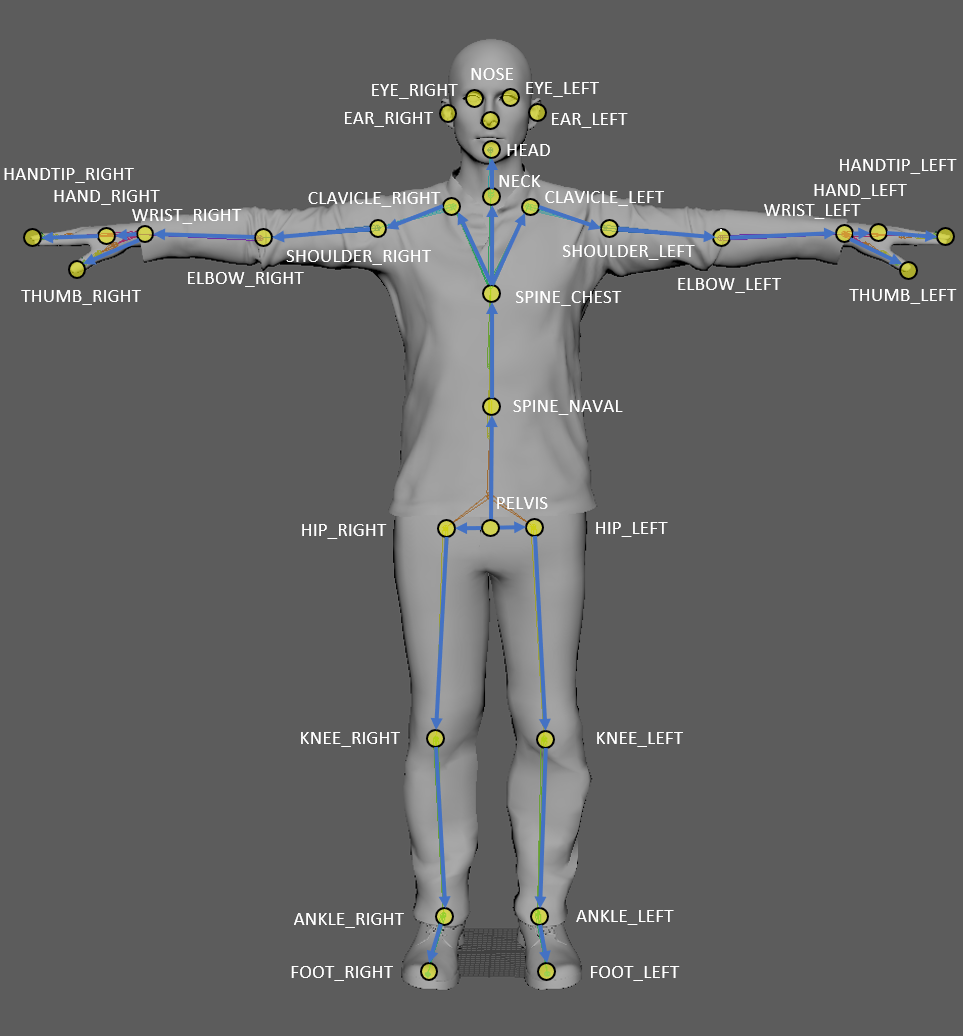
\includegraphics[width=0.70\textwidth]{images/loesungsweg/joint_hierarchy}
	\caption[Azure Kinect: 32 spezifische Positionen des menschlichen Körpers]{Azure Kinect: 32 spezifische Positionen des menschlichen Körpers \\Quelle: \cite{qm13_azure_joints_nodate}}
	\label{fig:joint_hierarchy}
\end{figure}
\FloatBarrier

Wie in Abbildung \ref{fig:joint_hierarchy} zu sehen ist, können bei der linken und rechten Hand unter anderem der Zeigefinger, Daumen, ca. die Mitte der Hand und das Gelenk über das Azure Kinect Body Tracking SDK, welches 32 spezifischen Positionen des menschlichen Körpers identifzieren kann, genutzt werden. Die Bestimmung und Nutzung der einzelnen Finger ist aufgrund der Limitierung des Azure Kinect Body Tracking SDKs und der verbauten Tiefenkamera der Azure Kinect nicht möglich. Aus diesem Grund können die einzelnen Finger mit der Azure Kinect nicht zur Gestensteuerung eines Industrieroboters eingesetzt werden. Deswegen wird auf feinmotorische Gesten, welche mit den einzelnen Fingern durchgeführt werden und zu denen z.B. das Skalieren mit zwei Fingern zählt, verzichtet \cite{qm13_azure_joints_nodate}. In der Tabelle \ref{tab:implementierte_gesten} sind die für die Gestensteuerung des Industrieroboters aufgestellten Gesten ersichtlich. Zum besseren Verständnis der Gesten wurden diese zudem mit den in Abbildung \ref{fig:joint_hierarchy} ersichtlichen 32 spezifischen Positionen des menschlichen Körpers, welche durch die Azure Kinect bereitgestellt werden, übersichtlich verknüpft. Bei der Entwicklung der Gesten wurde darauf geachtet, dass die Gesten für sowohl Links- aber auch Rechtshänder über die für das Teachen vorgesehene Zeit eine entspannte Möglichkeit bieten den Industrieroboter zu bedienen. Bei der Entwicklung der Gesten war es zudem sehr wichtig der bedienenden Person bei längeren Bedienungsvorgängen, wie z.B. der Gelenkstellung erhöhen, eine Möglichkeit zum Ablegen der Hände zu bieten um so Ermüdungserscheinungen vorbeugen zu können. Auf der anderen Seite war bei der Entwicklung der Gesten aber auch wichtig, diese in einer gewissen Distanz voneinander anzuordnen um so unbeabsichtigte Betätigungen mehrerer gleichzeitiger Gesten während des Bedienungsvorganges zu minimieren \cite{proff_radikale_2013}. Unbeabsichtigte Gesten können jedoch aber auch durch reflexartige Bewegungen zum Schutz des eigenen Leibes entstehen. Diese reflexartigen und unbeabsichtigten Gesten, wie z.B. das Schützen des Kopfes mit den Händen, \cite[95]{matschnig_korpersprache_2007} wurden bei der Entwicklung der Gesten mitberücksichtigt und werden von der entwickelten Roboter-Gesten-Anwendung größtmöglich herausgefiltert. Die Gesten in der Tabelle \ref{tab:implementierte_gesten} wurden aufgrund dieser Auswahlkriterien entwickelt, wobei deren Ergonomie in dieser Arbeit noch durch praxisnahe Teachvorgänge getestet werden muss. Bei allen in dieser Ausarbeitung entwickelten Gesten ist es entscheident, dass die bedienende Person Sichtkontakt zur Tiefenkamera und daher auch Sichtkontakt zum Industrieroboter hat um eine Aktion mit den entwickelten Gesten ausführen zu können. Bei Sichtunterbrechung zur Tiefenkamera oder bei Bestimmung mehrerer Personen im Blickfeld der Tiefenkamera wird die Bedienung des Industrieroboters mittels der Gesten zur Sicherheit deaktiviert. Ein Weiterarbeiten ist erst dann möglich, wenn die Sicht zur Tiefenkamera wiederhergestellt ist und sich nur noch eine einzige Person im Blickfeld der Tiefenkamera befindet.\newline

% ausführliche Begründung der implementierten Gesten für die jeweiligen Aktionen (Joint Mode, ...) und warum diese sinnvoll sind

\definecolor{LightGray}{gray}{0.9}
\definecolor{SeaShell}{rgb}{1.0, 0.96, 0.93}
\rowcolors{1}{}{SeaShell}

\begin{longtable}{|>{\raggedright\arraybackslash}p{0.175\textwidth}|>{\raggedright\arraybackslash}p{0.53\textwidth}|>{\raggedright\arraybackslash}p{0.19\textwidth}|}
\hline
\rowcolor{LightGray} \thead[c]{Aktion} & \thead[c]{Beschreibung\\mit\\spezifischer Geste} & \thead[c]{Anmerkung}\\
\hline
Gelenkstellung erhöhen & \textbf{Linker Zeigefinger} (\bracketText{HANDTIP\_LEFT}) kurz oder länger zwischen das \textbf{rechte Schlüsselbein} (\bracketText{CLAVICLE\_RIGHT}) und die \textbf{rechte Schulter} (\bracketText{SHOULDER\_RIGHT}) legen & \nameref{ast:gesten_anmerkung_1} \nameref{ast:gesten_anmerkung_4} \nameref{ast:gesten_anmerkung_5}\\
\hline
Gelenkstellung verringern & \textbf{Rechter Zeigefinger} (\bracketText{HANDTIP\_RIGHT}) kurz oder länger zwischen das \textbf{linke Schlüsselbein} (\bracketText{CLAVICLE\_LEFT}) und die \textbf{linke Schulter} (\bracketText{SHOULDER\_LEFT}) legen & \nameref{ast:gesten_anmerkung_1} \nameref{ast:gesten_anmerkung_4} \nameref{ast:gesten_anmerkung_5}\\
\hline
Position auf Weltachse erhöhen & \textbf{Linker Zeigefinger} (\bracketText{HANDTIP\_LEFT}) kurz oder länger zwischen das \textbf{rechte Schlüsselbein} (\bracketText{CLAVICLE\_RIGHT}) und die \textbf{rechte Schulter} (\bracketText{SHOULDER\_RIGHT}) legen & \nameref{ast:gesten_anmerkung_1} \nameref{ast:gesten_anmerkung_4} \nameref{ast:gesten_anmerkung_6}\\
\hline
Position auf Weltachse verringern & \textbf{Rechter Zeigefinger} (\bracketText{HANDTIP\_RIGHT}) kurz oder länger zwischen das \textbf{linke Schlüsselbein} (\bracketText{CLAVICLE\_LEFT}) und die \textbf{linke Schulter} (\bracketText{SHOULDER\_LEFT}) legen & \nameref{ast:gesten_anmerkung_1} \nameref{ast:gesten_anmerkung_4} \nameref{ast:gesten_anmerkung_6}\\
\hline
Endeffektor auseinanderfahren & \textbf{Rechter Zeigefinger} (\bracketText{HANDTIP\_RIGHT}) kurz oder länger in die \textbf{Mitte der Brusthöhe} (\bracketText{SPINE\_CHEST}) legen & \nameref{ast:gesten_anmerkung_1}\\
\hline
Endeffektor zusammenfahren & \textbf{Linker Zeigefinger} (\bracketText{HANDTIP\_LEFT}) kurz oder länger in die \textbf{Mitte der Brusthöhe} (\bracketText{SPINE\_CHEST}) legen & \nameref{ast:gesten_anmerkung_1}\\
\hline
Endeffektor-\newline Modus umschalten & \textbf{Linker Zeigefinger} (\bracketText{HANDTIP\_LEFT}) ca. für 2 s auf das \textbf{linke Knie} (\bracketText{KNEE\_LEFT}) legen \newline\newline \textbf{ODER} \newline\newline \textbf{rechter Zeigefinger} (\bracketText{HANDTIP\_RIGHT}) ca. für 2 s auf das \textbf{rechte Knie} (\bracketText{KNEE\_RIGHT}) legen & \nameref{ast:gesten_anmerkung_2} \newline\newline  Verfügbare Modi:\newline
$\bullet$ gesperrt\newline
$\bullet$ nicht gesperrt\newline\newline
Standardmäßig:\newline
$\bullet$ nicht gesperrt\\
\hline
Zum vorigen Gelenk wechseln & \textbf{Linker Zeigefinger} (\bracketText{HANDTIP\_LEFT}) kurz auf das \textbf{linke Ohr} (\bracketText{EAR\_LEFT}) oder das \textbf{linke Ohrläppchen} legen oder darüber schweben lassen & \nameref{ast:gesten_anmerkung_2}  \nameref{ast:gesten_anmerkung_3} \nameref{ast:gesten_anmerkung_5} \nameref{ast:gesten_anmerkung_7}\\
\hline
Zum nächsten Gelenk wechseln & \textbf{Rechter Zeigefinger} (\bracketText{HANDTIP\_RIGHT}) kurz auf das \textbf{rechte Ohr} (\bracketText{EAR\_RIGHT}) oder das \textbf{rechte Ohrläppchen} legen oder darüber schweben lassen & \nameref{ast:gesten_anmerkung_2}  \nameref{ast:gesten_anmerkung_3} \nameref{ast:gesten_anmerkung_5} \nameref{ast:gesten_anmerkung_7}\\
\hline
Zur vorigen Weltachse wechseln & \textbf{Linker Zeigefinger} (\bracketText{HANDTIP\_LEFT}) kurz auf das \textbf{linke Ohr} (\bracketText{EAR\_LEFT}) oder das \textbf{linke Ohrläppchen} legen oder darüber schweben lassen & \nameref{ast:gesten_anmerkung_2}  \nameref{ast:gesten_anmerkung_3} \nameref{ast:gesten_anmerkung_6}
\newline\newline Verfügbare Modi/Reihenfolge:\newline
$\bullet$ X (links/rechts)\newline
$\bullet$ Z (aufwärts/abwärts)\newline
$\bullet$ Y (vorwärts\newline /rückwärts)\newline\newline
Standardmäßig:\newline
$\bullet$ X (links/rechts)\\
\hline
Zur nächsten Weltachse wechseln & \textbf{Rechter Zeigefinger} (\bracketText{HANDTIP\_RIGHT}) kurz auf das \textbf{rechte Ohr} (\bracketText{EAR\_RIGHT})  oder das \textbf{rechte Ohrläppchen} legen oder darüber schweben lassen & \nameref{ast:gesten_anmerkung_2}  \nameref{ast:gesten_anmerkung_3} \nameref{ast:gesten_anmerkung_6}
\newline\newline Verfügbare Modi/Reihenfolge:\newline
$\bullet$ X (links/rechts)\newline
$\bullet$ Z (aufwärts/abwärts)\newline
$\bullet$ Y (vorwärts\newline /rückwärts)\newline\newline
Standardmäßig:\newline
$\bullet$ X (links/rechts)\\
\hline
Präzisions-\newline modus umschalten & \textbf{Linker Zeigefinger} (\bracketText{HANDTIP\_LEFT}) ca. für 2 s in den \textbf{Bereich des Bauchnabels} (\bracketText{SPINE\_NAVEL}) legen \newline\newline \textbf{ODER} \newline\newline \textbf{rechter Zeigefinger} (\bracketText{HANDTIP\_RIGHT}) ca. für 2 s in den \textbf{Bereich des Bauchnabels} (\bracketText{SPINE\_NAVEL}) legen & \nameref{ast:gesten_anmerkung_2} \newline\newline Verfügbare Modi:\newline
$\bullet$ präzise (Beschleunigung deaktiviert)\newline
$\bullet$ Beschleuni-\newline gung aktiviert\newline\newline
Standardmäßig:\newline
$\bullet$ präzise (Beschleunigung deaktiviert)\\
\hline
Positionen speichern & \textbf{Linker Zeigefinger} (\bracketText{HANDTIP\_LEFT}) ca. für 2 s auf die \textbf{linke Hüfthöhe} (\bracketText{HIP\_LEFT}) legen \newline\newline \textbf{ODER} \newline\newline \textbf{rechter Zeigefinger} (\bracketText{HANDTIP\_RIGHT}) ca. für 2 s auf die \textbf{rechte Hüfthöhe} (\bracketText{HIP\_RIGHT}) legen & \nameref{ast:gesten_anmerkung_2}\\
\hline
Koordinaten-\newline system-Modus umschalten & \textbf{Linker Zeigefinger} (\bracketText{HANDTIP\_LEFT}) kurz auf die \textbf{rechte Armbeuge} (\bracketText{ELBOW\_RIGHT}) legen \newline\newline \textbf{ODER} \newline\newline \textbf{rechter Zeigefinger} (\bracketText{HANDTIP\_RIGHT}) kurz auf die \textbf{linke Armbeuge} (\bracketText{ELBOW\_LEFT}) legen & \nameref{ast:gesten_anmerkung_2}
\newline\newline Verfügbare Modi:\newline
$\bullet$ Weltkoordinatensystem-Modus\newline
$\bullet$ Gelenk-Modus\newline\newline
Standardmäßig:\newline
$\bullet$ Weltkoordinatensystem-Modus\\
\hline
\hiderowcolors
\caption[Implementierte Gesten]{Implementierte Gesten\\Quelle: Eigene Ausarbeitung}
\label{tab:implementierte_gesten}\\
\showrowcolors
\end{longtable}

\paragraph*{$^{\ast1}$}\label{ast:gesten_anmerkung_1}\small{Wenn der Präzisionsmodus ausgeschalten ist (Beschleunigung aktiviert), führt ein längeres verharren in dieser Pose zu einer Beschleunigung der jeweiligen Bewegung.}\vspace{-0.75em}
\paragraph*{$^{\ast2}$}\label{ast:gesten_anmerkung_2}\small{Längeres verharren in dieser Pose ändert die Einstellung nur einmal. Um die Einstellung mehrmals zu ändern muss die Pose verlassen und anschließend neu initiiert werden.}\vspace{-0.75em}
\paragraph*{$^{\ast3}$}\label{ast:gesten_anmerkung_3}\small{Die Anzahl der Gelenke sind vom jeweiligen Industrieroboter abhängig.}\vspace{-0.75em}
\paragraph*{$^{\ast4}$}\label{ast:gesten_anmerkung_4}\small{Die Bewegung ist Abhängig von der Ausrichtung des Koordinatensystem des ausgewählten Gelenks/Weltachse.}\vspace{-0.75em}
\paragraph*{$^{\ast5}$}\label{ast:gesten_anmerkung_5}\small{Die Geste ist nur im Gelenk-Modus verfügbar. Die Aktion ist daher abhängig vom verwendeten Koordinatensystem-Modus.}\vspace{-0.75em}
\paragraph*{$^{\ast6}$}\label{ast:gesten_anmerkung_6}\small{Die Geste ist nur im Weltkoordinatensystem-Modus verfügbar. Die Aktion ist daher abhängig vom verwendeten Koordinatensystem-Modus.}\vspace{-0.75em}
\paragraph*{$^{\ast7}$}\label{ast:gesten_anmerkung_7}\small{Das standardmäßig ausgewählte Gelenk und die Reihenfolge beim Wechseln der Gelenke ist abhängig vom jeweiligen Industrieroboter.}\vspace{-0.75em}
\newline\newline

In der Tabelle \ref{tab:implementierte_gesten} sind die Aktionen, welche vom Industrieroboter ausgeführt werden können und mit Gesten verknüft wurden, aufgelistet. Bei der Entwicklung der Gesten wurden die erarbeiteten Auswahlkriterien für Gesten beachtet und bei den Gesten miteinbezogen. Bei längeren Aktionen, wie z.B. die Gelenkstellung erhöhen oder verringern, wurde darauf geachtet diese Aktionen mit möglichst angenehmen Gesten zu verknüpfen, welche es erlauben die Hände abzulegen. Dies beugt den Ermüdungserscheinungen von Gestenerkennungen vor, da der bedienenden Person eine Möglichkeit zum Ausruhen zur Verfügung gestellt wird. Zu jeder Geste wird in der Tabelle \ref{tab:implementierte_gesten} eine genaue Beschreibung angegeben um diese ordnungsgemäß nach der Anleitung ausführen zu können. In manchen Fällen, wie z.B. beim Umschalten des Präzisionsmodus, kann dies je nach Präferenz durch die linke oder rechte Hand erfolgen. Hierdurch steht es der Person frei die Geste seiner Wahl für den jeweiligen Anwendungsfall auszuwählen. Zur Erhöhung der Sicherheit wurde des Weiteren eine Möglichkeit implementiert den Endeffektor zu sperren um keine weiteren Aktionen mit ihm ausführen zu können. Z.B. wenn der Endeffektor eine Last transportiert ist es wichtig, dass die Last nicht plötzlich durch ungewolltes Öffnen des Endeffektors fallen gelassen wird. Dies würde ansonsten einen ungewollten Schaden verursachen. Standardmäßig ist der Endeffektor nicht gesperrt, da im Normalfall am Anfang noch keine Last transportiert wird. Der Präzisionsmodus ermöglicht das Wechseln zwischen einem präzisen Modues mit immer gleich bleibender Geschwindigkeit, welche für den jeweiligen Industrieroboter voreingestellt ist, und einem unpräziseren Modus, welcher aber dafür eine Beschleunigung der Bewegung bis zu einem für den Industrieroboter vorgegebenen Schwellwert, ermöglicht.

\begin{figure}[htb]
	\centering
	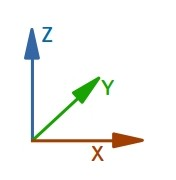
\includegraphics[width=0.2\textwidth]{images/loesungsweg/ros_coordinate_system}
	\caption[Kartesisches Koordinatensystem von ROS]{Kartesisches Koordinatensystem von ROS\\Quelle: Eigene Darstellung, in Anlehnung an \cite{guo_irc-set_2019}}
	\label{fig:ros_coordinate_system}
\end{figure}
\FloatBarrier

Zur Berechnung von Koordinaten im entsprechenden Koordinatensystem verwendetet ROS hierfür das kartesische Koordinatensystem, welches in Abbildung \ref{fig:ros_coordinate_system} ersichtlich ist \cite{guo_irc-set_2019}. Im implementierten Weltkoordinatensystem-Modus der Roboter-Gesten-Anwendung werden die Bewegungen daher im Bezug zu den Weltachsen durchgeführt. Die in der Tabelle \ref{tab:implementierte_gesten} erwähnten Weltachsen X, Y und Z entsprechen hierbei den Achsenbezeichnungen, welche in Abbildung \ref{fig:ros_coordinate_system} zu sehen sind. Die in der Tabelle \ref{tab:implementierte_gesten} aufgezeigten Gesten wurden für ähnliche Aktionen wiederverwendet um das Erlernen der Gesten zu errleichtern und die Bedienung intuitiv zu gestalten. Die Aktionen für die Gelenkstellung (\quoteMark{Gelenkstellung erhöhen} und die Position auf der Weltachse (\quoteMark{Position auf Weltachse erhöhen}, \quoteMark{Position auf Weltachse verringern}) zu verändern wurden vereinheitlicht, sowie die Aktionen um zwischen Gelenken zu wechseln (\quoteMark{Zum vorigen Gelenk wechseln}, \quoteMark{Zum nächsten Gelenk wechseln}) und zum Wechseln zwischen Weltachsen (\quoteMark{Zur vorigen Weltachse wechseln}, \quoteMark{Zur nächsten Weltachse wechseln}) wurden angeglichen.

\subsection{Sicherheitskonzept} % Sicherheitsvorkehrungen
Obwohl die implementierten Gesten so ausgelegt wurden, dass reflexartige und unbeabsichtigte Gesten weitaus unwahrscheinlicher als korrekte Gesten identifiziert werden, sollte nichtsdestotrotz auf keinen Fall auf den \quoteMark{Dead Man's Switch} verzichtet werden. Der \quoteMark{Dead Man's Switch} schützt im Extremfall die bedienende Person vor dem Industrieroboter bei fälschlicherweise als korrekt erkannten Gesten und ist daher unverzichtbar zum Schutz des eigenen Leibes. Eine ergonomische Lösung für die Form und Art des \quoteMark{Dead Man's Switch} zu finden würde jedoch über den Rahmen dieser Arbeit hinausgehen, da das Designen eines ergonomischen und sicheren \quoteMark{Dead Man's Switch} bereits eine Herausforderung für sich selbst darstellt. In dieser Arbeit wurde daher auf den \quoteMark{Dead Man's Switch} verzichtet, da die Ergonomie der Gesten und das Erkennen von Engpässen im Bezug auf die Übertragungslatenzen im Vordergrund stehen. Zudem wird bereits mit der Tiefenkamera überprüft ob die bedienende Person bei Gestenausführung zum Industrieroboter und dadurch auch zur Tiefenkamera schaut. Zudem stellt der \quoteMark{WidowX 200}-Lernroboter aufgrund seiner Größe, Beschleunigung und maximaler Geschwindigkeit keine lebensbedrohliche Gefahr für Menschen dar. Bei Verwendung der entwickelten Roboter-Gesten-Anwendung mit Industrierobotern, welche eine zu starke Beschleunigung und Geschwindigkeit zulassen, wird aus diesem Grund auf den Einsatz eines sinnvollen Sicherheitskonzepts appeliert. Bei Problemen oder beim Schließen der entwickelten Roboter-Gesten-Anwendung kann angegeben werden ob der Industrieroboter aus Sicherheitsgründen in die Ausgangsposition zurückgefahren werden soll. Dies kann je nach Industrieroboter unterschiedlich sinnvoll sein um z.B. beim \quoteMark{WidowX 200}-Lernroboter ein Zusammenstürzen des Lernroboters zu verhindern, da die Servo-Motoren des \quoteMark{WidowX 200}-Lernroboters nur bei angelegter Spannung die Position halten können. Bei praxisnahen Industrierobotern ist es zumeist nur sinnvoll den Industrieroboter bei Problemen mit der entwickelten Roboter-Gesten-Anwendung in seine Ausgangsposition zurückzuführen, wenn der Industrieroboter über einen Kamera besitzt um die bedienende Person nicht ungewollt zu verletzten. Diese Möglichkeit sollte daher mit Bedacht hinsichtlich der Sicherheit der bedienenden Person gewählt werden. Standardmäßig ist diese Option zur höhreren Sicherheit der bedienenden Person daher deaktiviert.

% Notstop-Handgerät: beim Erschrecken zu starkes drücken erkenne und ansonsten etwas bewusst drücken

\section{Aufbau des Roboter-Gesten-Frameworks}
Die in dieser Arbeit entwickelte Roboter-Gesten-Anwendung baut auf dem Roboter-Gesten-Framework, welches zusätzlich in dieser Arbeit erstellt wurde, auf. Der Vorteil des Roboter-Gesten-Frameworks besteht darin, dass durch dessen Einsatz die Entwicklung von einer Anwendung zur Gestensteuerung vereinfacht und dadurch auch beschleunigt wird. Das Roboter-Gesten-Framework bietet neben der Möglichkeit vordefinierte Gestenerkennungsalgorithmen, welche unter anderem Vektorberechnungen auf Basis der Tiefenkamerainformationen durchführen, zu verwenden, auch die Möglichkeit an um Industrieroboter über eine einheitliche Schnittstelle ansprechen zu können. Die Gestensteuerung kann jedoch unabhängig von einem Roboter und ROS erfolgen, da die Gesten- und Roboterkomponenten lose gekoppelt wurden und so mit verschiedenen Systemkonstellationen zusammenarbeiten können. Die Roboter-Gesten-Anwendung wurde als Demonstrationsanwendung entworfen um eine mögliche Nutzung des Roboter-Gesten-Frameworks vorzuzeigen.

\begin{figure}[htb]
	\centering
	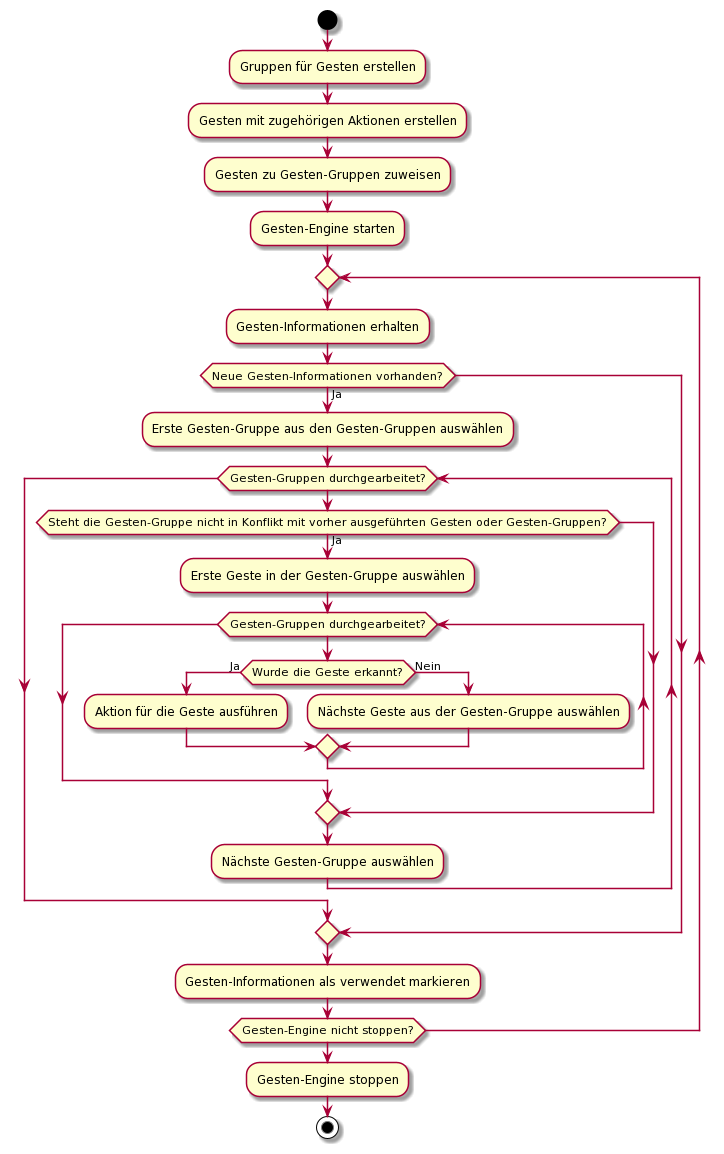
\includegraphics[width=0.85\textwidth]{images/loesungsweg/gesture_subsystem_uml}
	\caption[Gesten-Subsystem (Aktivitätdiagramm)]{Gesten-Subsystem (Aktivitätdiagramm)\\Quelle: Eigene Darstellung}
	\label{fig:gesture_subsystem_uml}
\end{figure}
\FloatBarrier

Das Gesten-Subsystem, dessen Ablauf in Abbildung \ref{fig:gesture_subsystem_uml} ersichtlich ist, verwaltet die zugewiesenen Gesten und deren auszuführende Aktionen. Die Gesten können dabei in sogenannte Gesten-Gruppen unterteilt werden um die Gesten einer kategorischen Gliederung zu unterwerfen. Zudem bieten die Gesten-Gruppen den Vorteil, dass ähnliche Gesten oder gegensätzliche Aktionen auf unkomplizierte Art und Weise voneinander isoliert werden können. Hierzu können Gesten in Gesten-Gruppe eingegliedert und Gesten und Gesten-Gruppen Prioritäten zugewiesen werden. Neben der Zuweisung von Prioritäten können Gesten auch individuelle Ausschlusskriterien zugeordnet werden. Die Gesten-Engine stellt zudem sicher, dass die gleichen Informationen, welche von der Tiefenkamera übertragen werden, nicht mehrmals wiederverwendet werden. Da Aktionen in Gesten-Gruppen zueinander gegensätzlich sein können, kann auch spezifiert werden ob mehrere Gesten für beide Hände zur gleichen Zeit erkannt werden können.

\begin{figure}[htb]
	\centering
	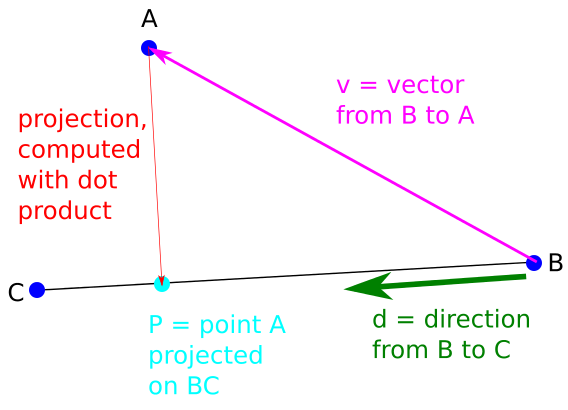
\includegraphics[width=0.55\textwidth]{images/loesungsweg/perpendicular_distance_illustration}
	\caption[Abstandsberechnung für Gestenerkennung]{Abstandsberechnung für Gestenerkennung
	\\Quelle: \cite{geometry_perpendicular_distance_nodate}}
	\label{fig:perpendicular_distance_illustration}
\end{figure}
\FloatBarrier

In Abbildung \ref{fig:perpendicular_distance_illustration} wird einer der Gestenerkennungsalgorithmen zur Erkennung der Distanz zwischen einem räumlichen Punkt zu einer Linie visualisiert. Dieser Algorithmus kann z.B. dazu genutzt werden um zu erkennen ob sich eine Hand in einem gewissen Bereich befindet. Dies kann sinnvoll sein um unbeabsichtigte Bewegungen außerhalb eines nicht spezifizierten Bereichs zu unterbinden. Hierzu wird zuerst der Punkt A auf die Linie von Punkt B zu Punkt C projiziert. Dieser neue Punkt P hat die geringste Distanz von Punkt A zur Linie BC und zudem steht die Linie AP lotrecht auf die Linie BC. Der neue Punkt P kann nun dazu genutzt werden um die Distanz zwischen P und A zu berechnen. Diese Distanz kann anschließend dazu genutzt werden um aufgrundlage der maximalen und minimalen Distanz des Bereichs zu entscheiden ob die Geste in einem erlaubten Bereich ausgeführt wurde. In mathematischer Schreibweise kann die Abbildung \ref{fig:perpendicular_distance_illustration} auch verkürzt als $\biggl| \frac{| \overrightarrow{BA} \times \overrightarrow{BC} |}{| \overrightarrow{BC} |} \biggl|$ dargestellt werden.

\begin{figure}[htb]
	\centering
	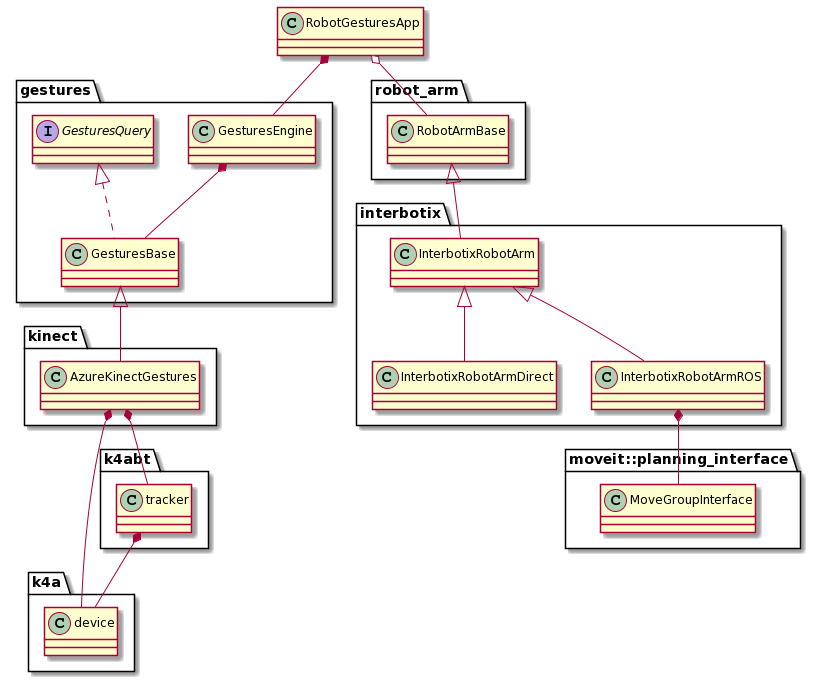
\includegraphics[width=0.75\textwidth]{images/loesungsweg/gesture_robot_system_uml}
	\caption[Modularität der Roboter-Gesten-Anwendung]{Modularität der Roboter-Gesten-Anwendung\\Quelle: Eigene Darstellung}
	\label{fig:gesture_robot_system_uml}
\end{figure}
\FloatBarrier

Die Roboter-Gesten-Anwendung wurde mit dem Roboter-Gesten-Framework erstellt und nutzt daher dieses als Grundlage, wie in Abbildung \ref{fig:gesture_robot_system_uml} mithilfe der \quoteMark{gestures}- und \quoteMark{robot\_arm}-Pakete visualisiert wurde. In dieser Anwendung wurden zudem die ausgewählten Gesten mithilfe der Gestenerkennungsalgorithmen des Roboter-Gesten-Frameworks umgesetzt. Hierzu verwendet es die vom Roboter-Gesten-Framework angebotenen Programmierschnittstellen um die Azure Kinect und den \quoteMark{WidowX 200}-Lernroboter, welcher über ROS oder eine direkte Kommunikation angesteuert werden kann, miteinander kommunizieren lassen zu können. Um vergleichbare Kommunikationsimplementierungen für ROS und die direkte Kommunikation mit dem \quoteMark{WidowX 200}-Lernroboter gewährleisten zu können, musste für den \quoteMark{WidowX 200}-Lernroboter das \quoteMark{InterbotiX}-SDK um eine direkte Kommunikation erweitert werden. Hierfür wurden die vom Roboter-Gesten-Framework bereitgestellten Programmierschnittstellen, wie z.B. die \quoteMark{GesturesBase}-Klasse und das \quoteMark{GesturesQuery}-Interface, verwendet um die einheitliche Kommunikation mit dem \quoteMark{WidowX 200}-Lernroboter zu realisieren. Für den \quoteMark{WidowX 200}-Lernroboter und die Azure Kinect wurden daher die entsprechenden Programmierschnittstellen für die Roboter-Gesten-Anwendung implementiert. Die genannte Klassenhierarchie und Vererbungsmöglichkeiten in Abbildung \ref{fig:gesture_robot_system_uml} ermöglicht jedoch die Unterstützung beliebiger Roboter und Tiefenkameras, solange die entsprechenden Programmierschnittstellen implementiert werden.\\

\begin{figure}[!h]
    \tikzstyle{block} = [draw, fill=green!18, rectangle, minimum height=3em, minimum width=6em]
    \tikzstyle{sum} = [draw, fill=green!18, circle, node distance=2cm]
    \tikzstyle{input} = [coordinate]
    \tikzstyle{output} = [coordinate]
    \tikzstyle{pinstyle} = [pin edge={to-,thin,black}]

    \tikzstyle{main} = [rounded corners, fill=yellow!20, minimum width=6.0cm, minimum height=7.1cm, text top]
    \tikzstyle{submain} = [node distance=0.9cm]

    \centering
    \begin{tikzpicture}[auto, node distance=4.3cm,>=latex']
        \node (people)[main, draw, rectangle] {Mensch};

        % We start by placing the blocks
        \node [input, submain, above left=-1.6cm and -0.45cm of people, name=input] {};
        \node [sum, right of=input, submain] (sum) {};
        \node [block, right of=sum, name=u, align=center, xshift=-1.1cm] (controller) {Regler};
        \node [block, right of=controller, name=u, align=center, xshift=-0.25cm, fill=red!20] (app) {Roboter-\\Gesten-\\Anwendung};
        \node [block, right of=app, pin={[pinstyle]above:Störungen},
                node distance=4.6cm] (system) {Roboter};
        % We draw an edge between the app and system block to
        % calculate the coordinate u. We need it to place the measurement block.
        \draw [->] (app) -- node[name=u, align=center] {Posen-\\änderungs-\\vorgabe} (system);
        \node [output, right of=system, xshift=-1.8cm] (output) {};
        \node [block, below of=controller] (measurements) {Messsystem};

        % Once the nodes are placed, connecting them is easy.
        \draw [draw,->] (input) -- node {} (sum);
        \draw [->] (sum) -- node[align=center] {e (Differenz\\in mm)} (controller);
        \draw [->] (controller) -- node[align=center] {Geste} (app);
        \draw [-] (system) -- node[name=y, align=center] {Ist-\\pose}(output);
        \draw [->] (output) |- (measurements);
        \draw [->] (measurements) -| node[pos=0.99] {-}
            node [near end] {} (sum);
    \end{tikzpicture}\newline
    \caption[Regelkreis der Roboter-Gesten-Anwendung]{Regelkreis der Roboter-Gesten-Anwendung\\Quelle: Eigene Darstellung}
    \label{fig:regelkreis_tir}
\end{figure}\FloatBarrier

Der Industrieroboter wird über den Mensch, welcher in dieser Arbeit die bedienende Person ist, mithilfe der Roboter-Gesten-Anwendung bewegt. Dieser Datenfluss kann mit dem Regelkreis in Abbildung \ref{fig:regelkreis_tir} visualisiert werden. Bei einer korrekt erkannten Eingabe des Menschen werden die Gelenke des Industrieroboters auf die notwendige Art und Weise eingestellt um die gewünschte Zielpose zu erreichen. Hierbei fungiert der Mensch, wie in Abbildung \ref{fig:regelkreis_tir} zu sehen ist, als Regler und die Roboter-Gesten-Anwendung als Stellsystem. Störungen, wie z.B. Gelenkungenauigkeiten, können dazu führen, dass der Roboter die gewünschte Pose nicht wie gewünscht erreicht. Der Mensch korrigiert deswegen die Pose des Industrieroboters solange bis die gewünschte Zielpose für den Anwendungsfall präzise genug erreicht wurde. Die Messung der Zielpose kann dabei z.B. über eine Schätzung oder ein genaues Ablesen in einer Simulationsumgebung über den Mensch erfolgen.

% ROS-Dependency Tree
% Tiefenkamera (Mindestanfordungen)

\section{Messvoraussetzungen}
Zur Messung der Übertragunslatenz bei der Gestensteuerung und zum anderen bei der Anbindung mit oder ohne ROS müssen die Messvoraussetzungen für die Replizierbarkeit zuerst klargestestellt werden. Die Messungen und deren Visualierungen basieren auf den Best Practices, welche im wissenschaftlichen Artikel \quoteMark{Ten Simple Rules for Effective StatisticalPractice} veröffentlicht wurden. Diese Regeln des wissenschaftlichen Artikels lauten wie folgt \cite{kass_ten_2016}:
\begin{compactenumerate}
    \item \textbf{Statistische Methoden sollten Daten ermöglichen, wissenschaftliche Fragen zu beantworten}: Es soll nicht auf der Struktur der Daten sondern aufgrundlage des wisschenschaftlichen Ziels der Daten gearbeitet werden. Z.B. können Daten aus einer Tabelle nach unterschiedlichen Aspekten klassifiziert werden anstatt diese direkt zu verwenden.
    \item \textbf{Signale sind rauschbehaftet}: Analoge Signale sind immer rauschbehaftet, da dies ein kontinuierliches Signal darstellt, und das Messen von physikalischen Größe immer mit Messfehlern behaftet ist.
    \item \textbf{Vorausplanen}: Es ist sinnvoll sich im Vorhinein Fragen zu stellen, welche den möglichen Ausgang der Messergebnisse betreffen. Zudem ist es auch hilfreich sich die möglichen Störgrößen klarzumachen um mögliche Probleme im Vorhinein zu lösen.
    \item \textbf{Über die Datenqualität nachdenken}: Es sollte überprüft werden ob die Daten vollständig sind, Anomalien in den Daten auftauchen und die Daten bereits vorbehandelt wurden.
    \item \textbf{Statistische Analyse ist mehr als eine Reihe von Berechnungen}: Es ist entscheident, dass die analythische Technik in geeigneter Weise mit den zu beantwortenden Fragen verknüpft ist. Daher sollte die Wahl der statischen Methode ausreichend begründet werden.
    \item \textbf{Simplizität (KISS)}: Eine große Anzahl von Messungen, Nachbearbeitungsmethoden oder ähnlichem kann zu einem starken Anstieg der Komplexität führen. Daher sollten die Daten und Messvorgänge so aufbereitet werden, dass diese nachvollziehbar und reproduzierbar sind.
    \item \textbf{Bewertung der Variabilität}: Je nach unterschiedlichen Umgebungskriteren bei den Messungen können mitunter Fehler nicht vollständig ausgeschlossen werden. Es ist sinnvoll die Daten hinsichtlich vorhandener Fehler zu hinterfragen.
    \item \textbf{Überprüfen der Annahmen}: Es sollten die Annahmen überprüft werden und bei Abweichungen sollten diese begründet werden können.
    \item \textbf{Wenn möglich replizieren}: Die Messungen sollten mehrmals in unterschiedlichen Testsituationen durchgeführt werden um so die Robustheit der Daten sicherstellen zu können.
    \item \textbf{Analyse reproduzierbar machen}: Die Ergebnisse sollten nachvollziehbar gestaltet werden, sodass diese von Dritten auf die gleiche Art und Weise repliziert werden können.
\end{compactenumerate}

Die Azure Kinect wird in einer Höhe von \num{0,85} m in einer zur Oberfläche geraden Ausrichtung positioniert. Der Abstand der testenden Person zur Azure Kinect beträgt mindestens \num{0,5} m bis zu maximal \num{1,80} m und die testende Person hat eine Körpergröße von \num{1,78} m. Der Testraum ist ein mit sonnenlicht belichteter Raum, welcher eine Raumtemperatur von \num{22,7} °C aufweist und die empfohlene Betriebsumgebung für die Azure Kinect aufweist \cite{tesych_azure_nodate}. Der Testrechner auf dem die Roboter-Gesten-Anwendung ausgeführt wird weist eine SSD und 8 GB RAM auf und hat einen AMD Ryzen 5 3600X 6-Kernprozessor, welcher über bis zu 12 logische Kerne verfügt, verbaut. Die Grafikkarte des Testsystems ist eine AMD Radeon RX 5700 XT wodurch das Body Tracking der Azure Kinect nur im CPU-Modus verwendet werden kann, da das Body Tracking der Azure Kinect nur CUDA basierte Nvidia Grafikkarten als Grafikkartenbeschleunigung zulässt \cite{encausse_body_nodate}. Der CPU-Modus des Azure Kinect Body Tracking SDK stellt daher der kleinste gemeinsame Nenner für alle Systeme dar und spiegelt so die Performance eines allgemein verfügbaren Systems wider.\\

Neben der Übertragungslatenz sind die genannten Messvoraussetzungen, aber auch für die Messung der Genauigkeit der erreichten Ziele und die Bestimmung der Ergonomie und User Experience erforderlich. Zur Messung der Genauigkeit der erreichten Ziele und zur Bestimmung der Ergonomie und User Experience wird ein möglichst praxisnaher Teachvorgang durchgeführt. Es soll eine Kontur so präzise wie möglich nachgefahren werden. Dabei ist zu beachten, dass in einem industriellen Szenario hierbei der Endeffektor z.B. für Laserschneiden ausgelegt sein könnte. Bei in dieser Arbeit durchgeführten Tests hingegen wird auf den Endeffektor des \quoteMark{WidowX 200}-Lernroboters zurückgegriffen.

\begin{figure}[htb]
	\centering
	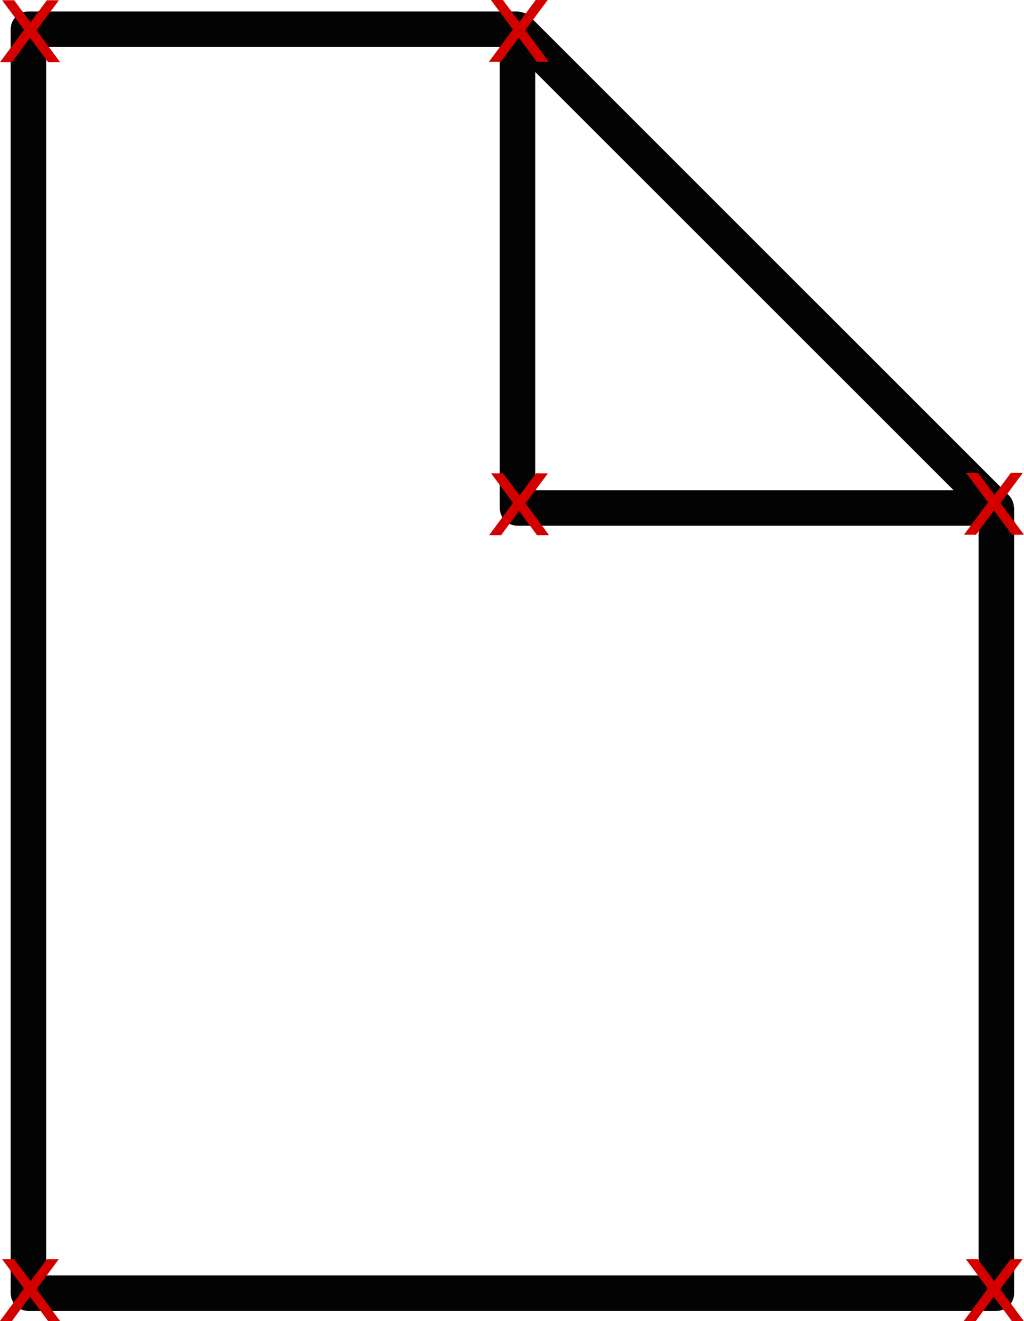
\includegraphics[width=0.25\textwidth]{images/loesungsweg/white-page-with-folded-corner}
	\caption[Teachbeispiel: Weiße Seite mit gefalteter Ecke]{Teachbeispiel: Weiße Seite mit gefalteter Ecke\\Quelle: Eigene Darstellung}
	\label{fig:white_page_with_folded_corner}
\end{figure}
\FloatBarrier

\begin{figure}[htb]
	\centering
	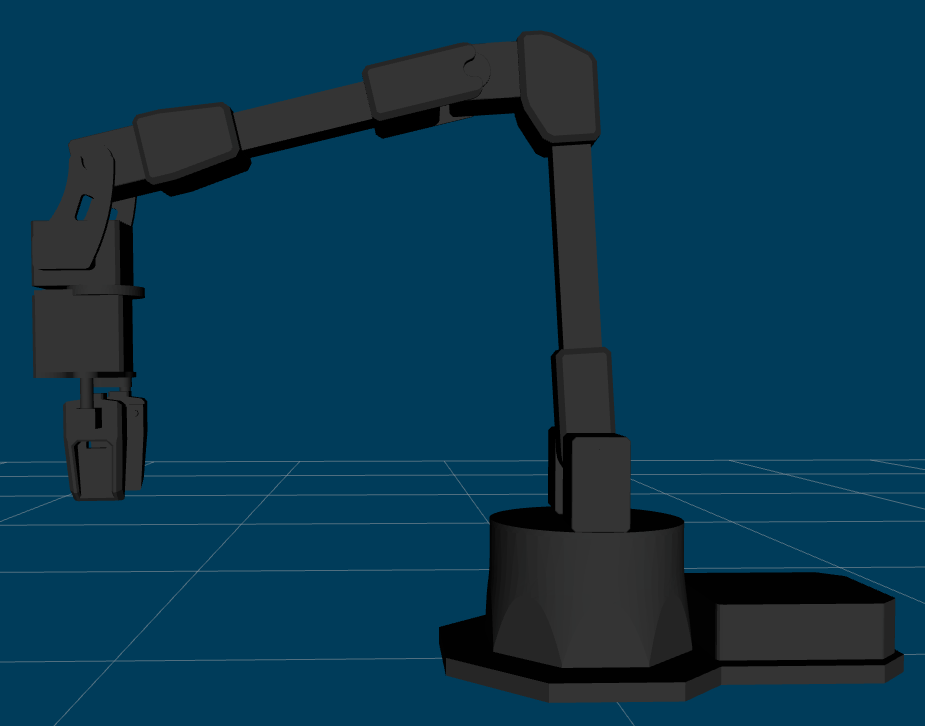
\includegraphics[width=0.65\textwidth]{images/loesungsweg/endeffektor_pose_2}
	\caption[Endeffektorpose für Testbeispiel]{Endeffektorpose für Testbeispiel\\Quelle: Eigene Darstellung}
	\label{fig:endeffektor_pose}
\end{figure}
\FloatBarrier

Zum Messen der Genauigkeit der anzufahrenden Ziele und zur Ermittlung der Genauigkeit der Gestenerkennung sollen die mit einem roten Kreuz markierten Positionen, wie in Abbildung \ref{fig:white_page_with_folded_corner} zu sehen sind, in der Simulationsumgebung Gazebo angefahren werden. Bei den durchzuführenden Messungen startet der \quoteMark{WidowX 200}-Lernroboter immer in seiner Standard-Ausgangsposition. Um die Kontur nachfahren zu können soll der Endeffektor aus der Anfangs schrägen Pose zuerst so wie in Abbildung \ref{fig:endeffektor_pose} positioniert werden. Daraufhin sollen die Mittelpunkte der rot markierten Kreuze mit dem Greifer angefahren werden, sodass der Mittelpunkt des Greifers über dem roten Kreuzpunkt liegt. Die Zeit zum Erreichen der Ziele und die Abweichung zu den Zielen werden über 10 Testläufe hinweg gesammelt und daraufhin ausgewertet werden. Die vorraussichtliche Durchlaufzeit für jeden Testlauf wird auf 15 Minuten geschätzt wodurch die Durchführung von 10 Testläufen ca. \num{2,5}-Stunden betragen wird. Diese Zeitdauer sollte ausreichen um zudem die Ergonomie ausreichend testen zu können. Um die Latenz der Gestenerkennung und der Kommunikation mit dem Roboter zu ermitteln und statistisch aussagekräftige Daten zu erhalten werden zudem Tests anhand eines realen \quoteMark{WidowX 200}-Lernroboters durchgeführt. Anzumerken ist, dass aufgrund der 5 DOF des \quoteMark{WidowX 200}-Lernroboters ist ein Teilbereich der Positionen des 3D-Raums nicht ansteuerbar. Hierfür würde wäre ein Industrieroboter mit mindestens 6 DOF notwendig. Im Weltkoordinatensystem-Modus kann es daher aufgrund der 5 DOF des \quoteMark{WidowX 200}-Lernroboters passieren, dass dieser seine Gelenkpositionen mit sehr großen Positionsändernungen, welche in sprunghaften Änderen des Roboters ersichtlich sind, anpassen muss um Positionen im 3D-Raum erreichen zu können.

\textcolor{red}{TODO:\\
realer Test aufheben von Objekt? wie groß \& wie schwer?\\
Größe der Seiten in Abbildung 3.3 hinzufügen\\
Weiteres Testbeispiel hinzufügen? Für Ergonomie Dinge aufheben?
}
% https://www.dnsstuff.com/network-latency-test-tools
